\documentclass[12pt]{iopart} % Document class declaration

% package "imports"
\usepackage{graphicx}
\usepackage{IEEEtrantools}
\usepackage{amsmath} % For centering equations

% Custom macros
\gdef\mcm{r@{.}l@{ ± }r@{.}l} % Multi Column Measurement; Used for decimal aligning & ± aligning
\gdef\mch#1{\multicolumn{4}{l}{#1}} % Multi Column Header; Used for decimal aligning & ± aligning
\gdef\mcmnd{r@{ ± }l} % Multi Column Measurement No Decimal; Used for ± aligning when the values don't need a decimal point
\gdef\mchnd#1{\multicolumn{2}{l}{#1}} % Multi Column Header No Decimal; Used for  ± aligning when the values don't need a decimal point
\gdef\sci#1#2{#1 \times 10^{#2}}
\gdef\units#1{~\mathrm{#1}}
\graphicspath{{./images/}}

%%%%%%%%%%%%%%%%%%%% Document Starts %%%%%%%%%%%%%%%%%%%%
\begin{document}

%%%%%%%%%%%%%%%%%%%% Title Page %%%%%%%%%%%%%%%%%%%%
\title{Realistic Projectiles}
\author{Ali Mortada, Xavier Valencia, James Phommachanh, Wes Cochran}
\vspace{10pt}
\begin{indented}
  \item[]Mt.~San Antonio College, ENGR 285, CRN 43464
  \item[]May 20, 2024
\end{indented}
\newpage

%%%%%%%%%%%%%%%%%%%% Objectives %%%%%%%%%%%%%%%%%%%%
\section{Objectives}

\begin{center}
\subtitle{\textbf{Interdependence of Motion}}
\end{center}

The quadratic air resistance model has motion that is interdependent, meaning that the horizontal and vertical motion are not independent of one another. 
This can be shown in the differential equations describing the horizontal and vertical motion of the model. 

\begin{equation} \label{eq:1}
    \frac{\mathrm{d}^2 x}{\mathrm{d}t^2} = -k \vec{v_x} \sqrt{v_x^2+v_y^2}
\end{equation}

\begin{equation} \label{eq:2}
  \frac{\mathrm{d}^2 y}{\mathrm{d}t^2} = \vec{g} -k \vec{v_y} \sqrt{v_x^2+v_y^2}
\end{equation}


Since the magnitude of the motion depends on both the horizontal and vertical motion, having a different vertical or horizontal initial motion would affect the motion of either component. 
The differential model cannot be solved by hand but can be shown numerically by plotting the result using the RK4 method. 
In this case, $\vec{g} = 1$ and $\vec{v_\infty} = 1$ (i.e $k = 1$) and to show a change in both components, the horizontal motion and vertical will be increased by a step of 3 three times. 
As a result, two graphs qualitatively show that the horizontal and vertical motion are not independent. 

% how to do el figure
%\begin{figure}[h!tbp]
%  \begin{center}
% \item[]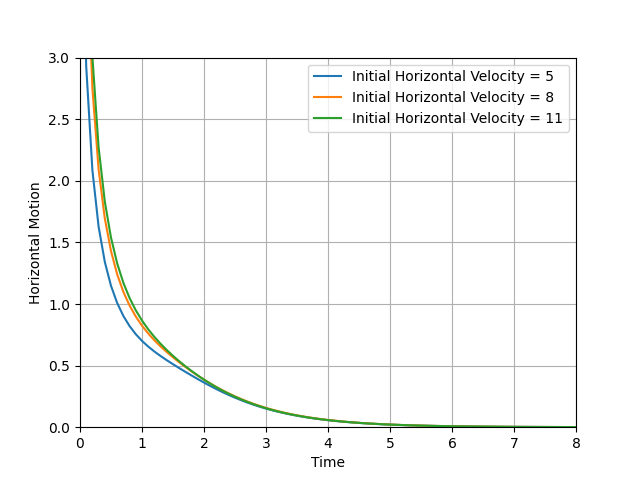
\includegraphics[width=0.6\textwidth]{figure1.png}
%  \caption{\label{fig:figure1}
%  Outcome one when \emph{energy\_gain} has the highest step with a random distribution.
%  }
%  \end{center}
%\end{figure}

\begin{figure}[h!tbp]
  \begin{center}
 \item[]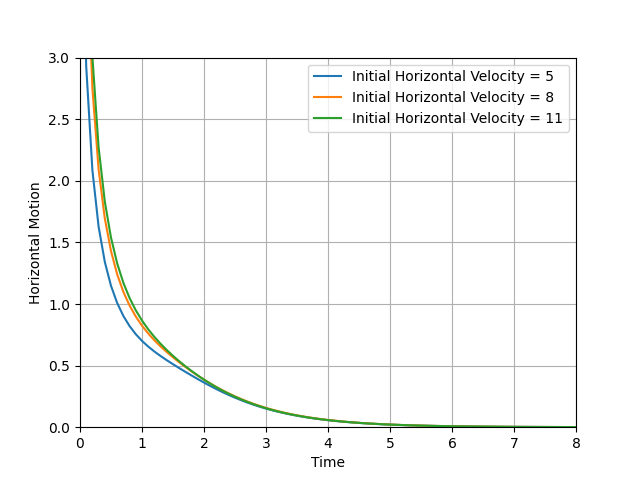
\includegraphics[width=0.6\textwidth]{figure1.png}
  \caption{\label{fig:figure1}
  Horizontal motion vs. time.
  }
  \end{center}
\end{figure}

\begin{figure}[h!tbp]
  \begin{center}
 \item[]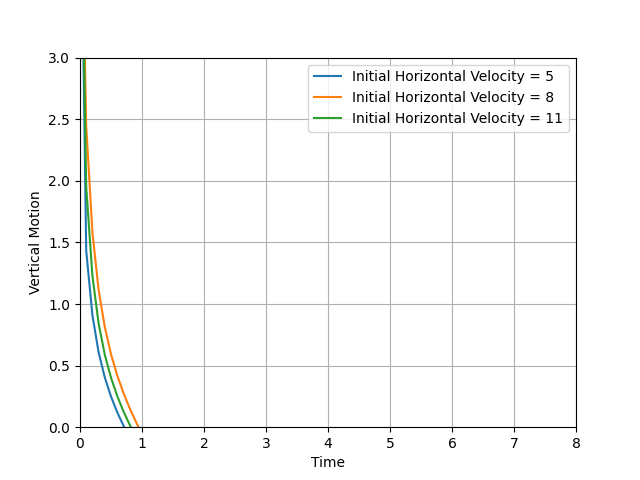
\includegraphics[width=0.6\textwidth]{figure2.png}
  \caption{\label{fig:figure2}
  Vertical motion vs. time.
  }
  \end{center}
\end{figure}

Changing the step in the horizontal motion can have effects in the vertical motion of the graph over time. 
This is directly based on the differential equations that model the motion. 
If the horizontal and vertical motion were independent, then changing the horizontal motion should not affect the vertical motion.

\pagebreak

\begin{center}
\subtitle{\textbf{Trajectories}}
\end{center}

The general shape of the projectile exhibits an elliptical shape based on the firing angle and the initial velocity. 
Fig \ref{fig:figure3} models the projectile against the vertical distance and horizontal distance at some initial angle and speed.

\begin{figure}[h!tbp]
  \begin{center}
 \item[]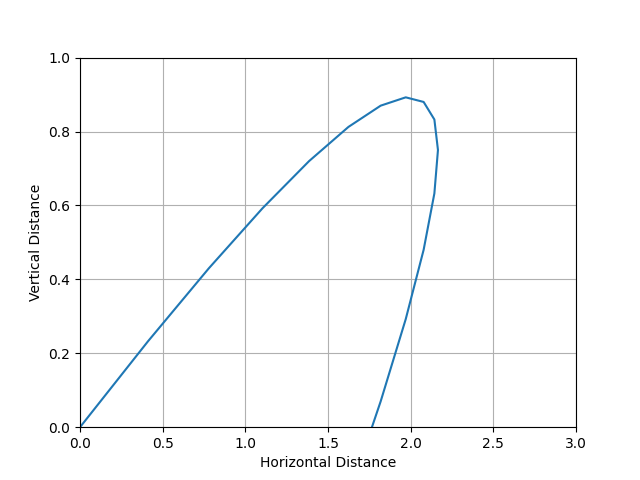
\includegraphics[width=0.6\textwidth]{figure3.png}
  \caption{\label{fig:figure3}
  General shape of the trajectory.
  }
  \end{center}
\end{figure}

The general shape of the projectile can change based on the initial speed and the initial angle. 
When the initial angle increases, the shape of the trajectory becomes steeper. 
The initial speed causes the projectile to go further when increased. 
The two figures below show this in greater detail with Figure \ref{fig:figure4} having the initial speed incremented by 0.5 and Figure \ref{fig:figure5} having an initial angle incremented by 10 degrees.

\begin{figure}[h!tbp]
  \begin{center}
 \item[]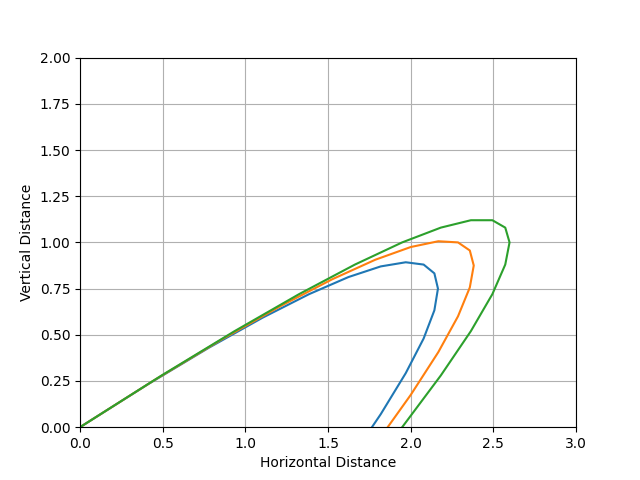
\includegraphics[width=0.6\textwidth]{figure4.png}
  \caption{\label{fig:figure4}
  Trajectory with an increasing initial speed.
  }
  \end{center}
\end{figure}

\begin{figure}[h!tbp]
  \begin{center}
 \item[]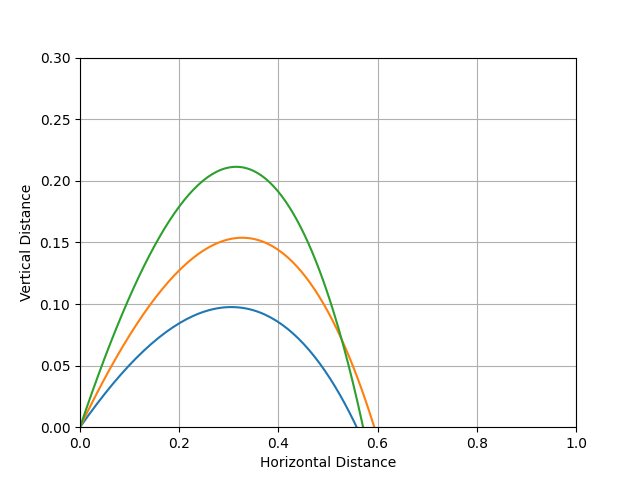
\includegraphics[width=0.6\textwidth]{figure5.png}
  \caption{\label{fig:figure5}
  Trajectory with an increasing initial angle.
  }
  \end{center}
\end{figure}

\pagebreak

\begin{center}
\subtitle{\textbf{Firing Range}}
\end{center}

Blah blah blah 3.


\pagebreak

%%%%%%%%%%%%%%%%%%%% Extension %%%%%%%%%%%%%%%%%%%%
\section{Extension: Incorporating Lift}

For the extension, we chose to incorporate a lift force that always points upwards and, similar to the drag force, increases quadratically with velocity.
This addition slightly modifies Eq. \ref{eq:2}, as there is now the lift constant, $\Gamma$, that controls the motion in the vertical direction.
Thus, this equation becomes:

\begin{equation} \label{eq:3}
  \frac{\mathrm{d}^2 y}{\mathrm{d}t^2} = \vec{g} + (\Gamma - k) \vec{v_y} \sqrt{v_x^2+v_y^2}
\end{equation}



\end{document}
%%%%%%%%%%%%%%%%%%%% Document Ends %%%%%%%%%%%%%%%%%%%%